% Options for packages loaded elsewhere
%\PassOptionsToPackage{unicode}{hyperref}
\PassOptionsToPackage{hyphens}{url}
%
\documentclass[ignorenonframetext,]{beamer}
\usepackage{pgfpages}
\setbeamertemplate{caption}[numbered]
\setbeamertemplate{caption label separator}{: }
\setbeamercolor{caption name}{fg=normal text.fg}
\beamertemplatenavigationsymbolsempty
% Prevent slide breaks in the middle of a paragraph
\widowpenalties 1 10000
\raggedbottom





\AtBeginSection{
	\begin{frame}
	\centering
	%{\usebeamerfont{section name}\usebeamercolor[fg]{section name}#1}
	\vskip1em\par
	\begin{beamercolorbox}[sep=12pt,center]{part title}
		\usebeamerfont{section title}\insertsection\par
	\end{beamercolorbox}	
	\end{frame}
}




\usepackage{lmodern}
\usepackage{amssymb,amsmath}
\usepackage{ifxetex,ifluatex}
\ifnum 0\ifxetex 1\fi\ifluatex 1\fi=0 % if pdftex
  \usepackage[T1]{fontenc}
  \usepackage[utf8]{inputenc}
  \usepackage{textcomp} % provide euro and other symbols
\else % if luatex or xetex
  \usepackage{unicode-math}
  \defaultfontfeatures{Scale=MatchLowercase}
  \defaultfontfeatures[\rmfamily]{Ligatures=TeX,Scale=1}
\fi

\usetheme[]{Madrid}
% Use upquote if available, for straight quotes in verbatim environments
\IfFileExists{upquote.sty}{\usepackage{upquote}}{}
\IfFileExists{microtype.sty}{% use microtype if available
  \usepackage[]{microtype}
  \UseMicrotypeSet[protrusion]{basicmath} % disable protrusion for tt fonts
}{}
\makeatletter
\@ifundefined{KOMAClassName}{% if non-KOMA class
  \IfFileExists{parskip.sty}{%
    \usepackage{parskip}
  }{% else
    \setlength{\parindent}{0pt}
    \setlength{\parskip}{6pt plus 2pt minus 1pt}}
}{% if KOMA class
  \KOMAoptions{parskip=half}}
\makeatother
\usepackage{xcolor}
\IfFileExists{xurl.sty}{\usepackage{xurl}}{} % add URL line breaks if available
%\IfFileExists{bookmark.sty}{\usepackage{bookmark}}{\usepackage{hyperref}}

%\hypersetup{
 % pdftitle={Analytics for campaigns},
  %pdfauthor={Valerie Bradley},
  %hidelinks,
  %pdfcreator={LaTeX via pandoc}}

\urlstyle{same} % disable monospaced font for URLs
%\newif\ifbibliography
\usepackage{graphicx,grffile}
\makeatletter
\def\maxwidth{\ifdim\Gin@nat@width>\linewidth\linewidth\else\Gin@nat@width\fi}
\def\maxheight{\ifdim\Gin@nat@height>\textheight\textheight\else\Gin@nat@height\fi}
\makeatother
% Scale images if necessary, so that they will not overflow the page
% margins by default, and it is still possible to overwrite the defaults
% using explicit options in \includegraphics[width, height, ...]{}
\setkeys{Gin}{width=\maxwidth,height=\maxheight,keepaspectratio}
% Set default figure placement to htbp
\makeatletter
\def\fps@figure{htbp}
\makeatother
\setlength{\emergencystretch}{3em} % prevent overfull lines
\providecommand{\tightlist}{%
  \setlength{\itemsep}{0pt}\setlength{\parskip}{0pt}}
\setcounter{secnumdepth}{-\maxdimen} % remove section numbering
%\setbeamertemplate{navigation symbols}{}
%ß\setbeamertemplate{footline}[frame number]{}

\usepackage{tikz}
\usepackage{colortbl}
\usepackage[]{algorithm2e}
\usepackage{pifont}
\usepackage{amssymb}


\newcommand\ci{\perp\!\!\!\perp}


\institute[University of Oxford]{University of Oxford, Department of Statistics}

\titlegraphic{
	\vspace{1cm}
	\includegraphics[width=3cm]{/Users/valeriebradley/Documents/Oxford/logos/ox_small_cmyk_pos_rect.png}
}

%\definecolor{oxfordblue}{rgb}{0.267, 0.412, 0.49}
\definecolor{oxfordblue}{rgb}{0, 0.129, 0.278}
\definecolor{oxfordlightblue}{RGB}{25, 56, 87}
\definecolor{oxfordred}{RGB}{186, 12, 47}
\definecolor{oxfordgreen}{RGB}{15,115,97}
\usecolortheme[named=oxfordblue]{structure}


\setbeamerfont{alerted text}{series=\bfseries}
\setbeamercolor{alerted text}{fg=oxfordblue}





\setbeamertemplate{section page}[mine]

\title{Machine learning methods for political campaigns}
\author{Valerie Bradley}
\date{15 November 2019}

\begin{document}
\begin{frame}
\titlepage
\end{frame}

\begin{frame}
  \tableofcontents[hideallsubsections]
\end{frame}

\section{Background}

\begin{frame}{My background}
\begin{columns}[t]
	\column{.5\textwidth}
	\centering
	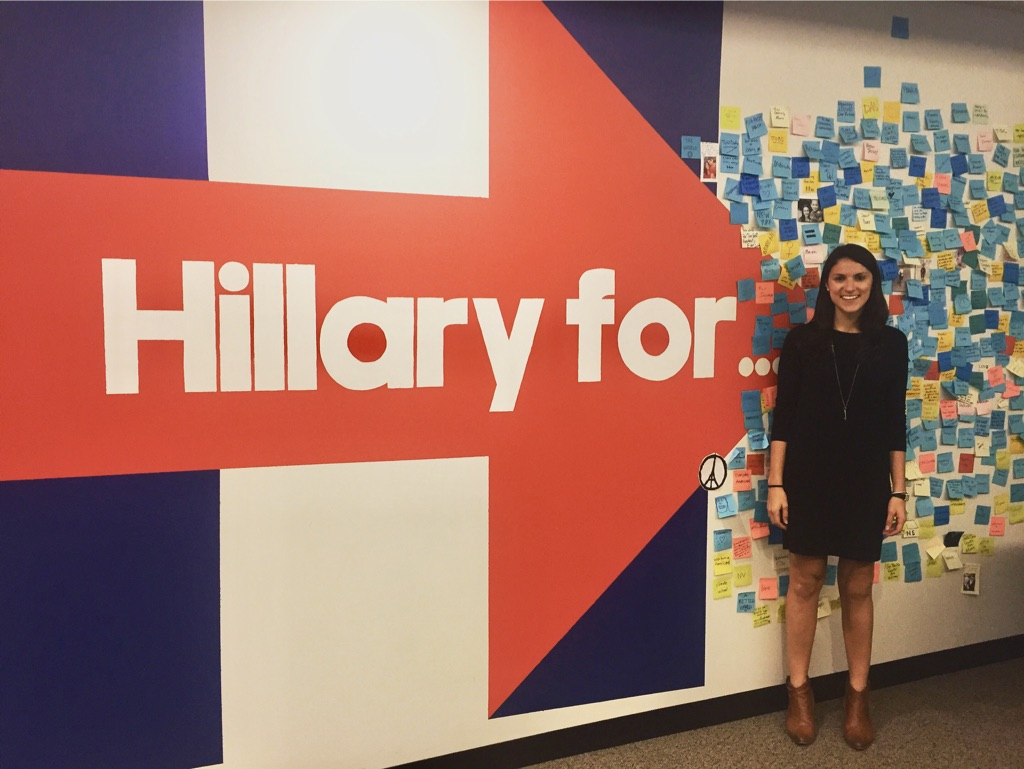
\includegraphics[width=5cm,height=3.5cm]{photos/hfa_1.jpg}\\
	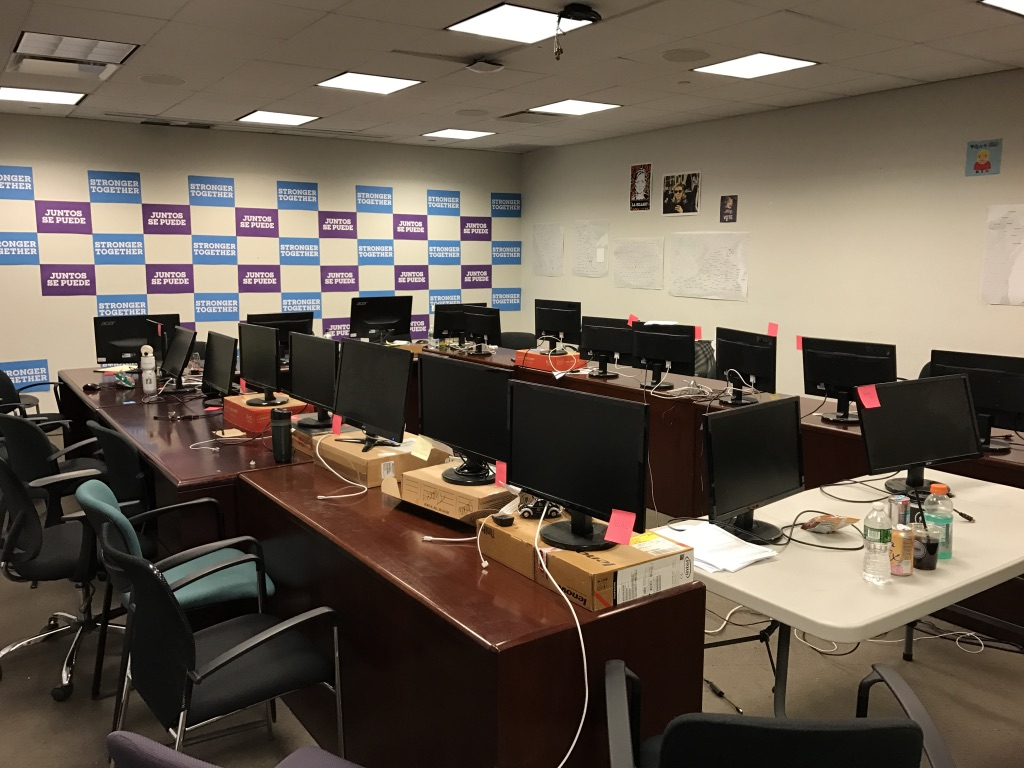
\includegraphics[width=5cm,height=4cm]{photos/hfa_enight_1.jpg}
	\column{.5\textwidth}
	\centering
	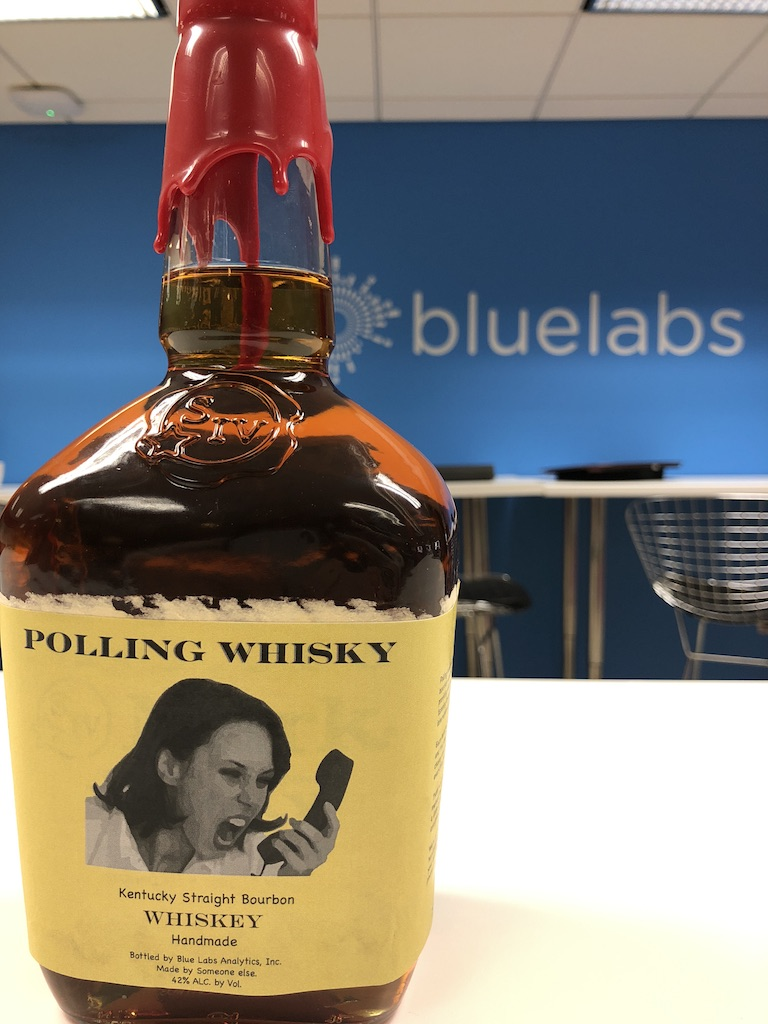
\includegraphics[width=5cm,height=4cm]{photos/bl_pollingwhiskey.jpg}\\
	
\includegraphics[width=5cm,height=4cm]{photos/bl_va.jpg}
\end{columns}
\end{frame}

\section{Political campaign analytics overview}

\begin{frame}{How are analytics used in campaigns?}
\textbf{Goal}: win more votes / seats / power than the other candidate(s)\\

\pause
Key questions for a campaign:
\pause
\begin{enumerate}
	\item<2-> \textbf{Current state of the race}. If we did nothing, who would win?
	\item<3-> \textbf{Develop ``path to victory"}. What do we have to do to move from current state of the race to winning state? Who do we have to persuade v. who do we have to make sure turns out to vote?
	\item<4-> \textbf{Optimization}.  How do we spend our budget (eg. across modes of outreach like TV, digital, mail, etc., or across targets within each mode) to maximize our impact on key demograpic groups / regions?
	\item<5-> \textbf{Tracking}.  Are we moving people?  Are we losing ground? Are we hitting goals?
\end{enumerate}
\end{frame}


\begin{frame}{The basic analytics products}

\pause
\begin{enumerate}
	\item State-of-the-race models:
	\begin{enumerate}
		\item \textbf{Turnout score}, $\hat{p}(T = 1|x_i)$
		\item \textbf{Support score}, $\hat{p}(Y = 1|x_i)$
	\end{enumerate}
\pause
	\item Behavior change models:
	\begin{enumerate}
		\item \textbf{Persuasion score}, $\hat{p}(P = 1 | x_i, Z = 1) = \hat{p}(Y = 1 | x_i, Z = 1) - \hat{p}(Y = 1 | x_i, Z = 0)$, \\where $Z$ is a treatment indicator
		\item \textbf{Get Out The Vote (GOTV) score} , $\hat{p}(T=1 | x_i, C = 1)$ \\where $C=1$ if contacted by the campaign
	\end{enumerate}
\pause
	\item Mode contactability / impact models
	\begin{enumerate}
		\item \textbf{Poll response rate models}: $\hat{p}(R= 1|x_i, \text{[attempted]})$
		\item \textbf{Impact models}: $\hat{p}(I = 1|x_i, \text{[recieve an ad]})$
	\end{enumerate}
	

\end{enumerate}




\end{frame}

\begin{frame}{The data}

Main sources of data:
\begin{itemize}
	\item<2-> \textbf{Voterfile}: List of all registered voters in the country (historical turnout data, registration address and phone number, age, gender, etc.)
	\item<3-> \textbf{Consumer and census data}: appended to the (publicly available) voterfile
	\item<4-> \textbf{Contact history data}: voter interaction data collected by campaigns over many election cycles
	\item<5-> \textbf{Historical results and scores}: most granular unit of results is precinct-level (approx. 1000-3000 registered voters), adjust previous scores to actual election results
	\item<6-> \textbf{Survey data}: data collected in-cycle on the current state of the race, either over the phone or online; different types of polls (modeling, tracking, message testing)
\end{itemize}
\end{frame}


\begin{frame}{Common problems}

Some common problems in political campaign analytics:
\begin{itemize}
	\item<2-> We never observe the outcome we try to predict (vote choice at the individual-level)
	\item<3-> Quality of polls and models judged by accuracy of e-day prediction, but the outcome used in training is observed at a different moment in time (and opinions change!)
	\item<4-> Contact history data is biased (collection is targeted using modeled scores)
	\item<5-> \alert<7->{Survey data is really expensive to collect (a single response costs 10-20 USD); people don't respond}
	\item<6-> \alert<7->{Standard supervised learning techniques require an outcome (eg. survey response) matched 1:1 to covariate data (eg. voterfile data), so the survey modes we can use are limited; harder with new data privacy restrictions}
\end{itemize}
\end{frame}


\section{Project 1: Methods for selection bias}

\begin{frame}{Methods for selection bias}
\textbf{Selection bias}: "preferential exclusion of units from samples" with unknown probability (Bareinboim, 2014). Interested in $\text{P}(y)$, but only observe $\text{P}(y|S = 1)$ and $Y \not \ci S$

\pause
\textbf{What can we do?}  Try to find a set of auxilary variables $\mathbf{Z}$ s.t. $Y\ci S|\mathbf{Z}$\\
\pause
Then, we can recover $\text{P}(y)$ with:
\begin{equation}\label{eq:recovery}
\text{P}(y) = \sum_\mathbf{z} \text{P}(y|\mathbf{z}, S=1)\text{P}(\mathbf{z})
\end{equation}


\end{frame}


\begin{frame}{Methods for selection bias}
Two main families of methods:
\pause
\begin{itemize}
	\item \textbf{Regression methods}: estimate $\text{P}(y|\mathbf{z}, S=1)$ then project regression model on population distribution $P(\mathbf{z})$\\
	\begin{itemize}
		\item	MRP (Mister P) is a \textbf{really} popular method in political science for this
	\end{itemize}
\pause
	\item \textbf{Inverse probability weighting (IPW)}: Estimate the probability of selection $\text{P}(S = 1 | \mathbf{z})$, then assign observations weights of $1/\hat{\text{P}}(S = 1|\mathbf{z})$ and use to calculate weighted estimate of $\text{P}(y)$.\\
	\pause This works because we can re-express Eq. \ref{eq:recovery}:
	\begin{align} \label{eq:IPSW}
	\text{P}(\mathbf{y}) &= \sum_\mathbf{Z} \text{P}(\mathbf{y}| \mathbf{z}, S=1)\text{P}(\mathbf{z})= \sum_\mathbf{Z} \text{P}(\mathbf{y}, \mathbf{z} | S = 1)\frac{\text{P}(S = 1)} {\textcolor{oxfordred}{\text{P}(S = 1 | \mathbf{z})}}
	\end{align}
\end{itemize}
\pause
\textbf{Problem}: What if $\mathbf{Z}$ is large?  Or contains continuous variables?

\pause
\textbf{Which to use?} Regression is flexible, but outcome dependent
\end{frame}

\begin{frame}{Estimating \(\text{P}(S = 1 | \mathbf{Z})\)}

Things to think about when comparing methods for estimating
\(\text{P}(S = 1 | \mathbf{Z})\):

\begin{enumerate}
	\item Weighted \textbf{marginal distribution} of \(\mathbf{Z}\) should match that of the population
	\item Avoid extreme weights that inflate the \textbf{variance} of estimators (have to account for the additional uncertainty of weights)
	\item \textbf{Computational complexity} of the method (weighting should be FAST, otherwise you should just build a model for $Y$)
	\item How well does the method account for \textbf{interactions} between elements of \(\mathbf{Z}\)
\end{enumerate}

\end{frame}


\begin{frame}{MANY IPW methods (I)}

Classic weighting methods:

\begin{enumerate}
	\item
	\emph{Post-stratification}: adjust to the joint distribution of \(\mathbf{Z}\) (exactly Eq \ref*{eq:IPSW})
	\item
	\emph{Raking}: iteratively adjust the marginal distributions of elements in \(\mathbf{Z}\)
	\item
	\emph{Calibration}: raking, but can handle continuous variables (use population totals of continuous variables as constraints)
\end{enumerate}

\pause
Less-common methods:

\begin{enumerate}
	\setcounter{enumi}{3}
	\item
	\emph{Logit}: estimate the $\text{P}(S = 1 | \mathbf{z})$ directly with regularized regression
	\item
	\emph{LASSO}: use a LASSO to select important subset of $\mathbf{Z}$, then rake to subset
\end{enumerate}

\end{frame}


\begin{frame}{MANY IPW methods (II)}
New methods:
\begin{enumerate}
	\setcounter{enumi}{5}
	\item \emph{BART + raking}: use a Bayesian Additive Regression Tree (BART)
	to estimate the probability of selection, then rake such that key
	marginal distributions match those of the population
	\pause
	\item \emph{Kernel Mean Matching (KMM)}: Estimate weights $\mathbf{w}$ that minimize distance in RKHS between sample ($s$) and population ($p$) covariate distributions
	\begin{align*}
	\underset{\mathbf{w}}{\operatorname{argmin}} & \left| \left| \frac{1}{n_{s}} \sum_{i = 1}^{n_{s}} w_i \phi(z_i^{s})  - \frac{1}{n_{p}} \sum_{i = 1}^{n_{p}} \phi(z^{p}_i) \right| \right| \\
	\text{subject to }& \mathbf{w} \in [0, B] \text{ and } \left| \sum_{i = 1}^{n_{s}} w_i - n_{s} \right| \leq n_{s}\epsilon
	\end{align*}
	\pause
	\item \emph{Post-stratification with} \texttt{k-means++}: Use \texttt{k-means++} to define strata for post-stratification
\end{enumerate}
\end{frame}

\begin{frame}{Some results}
\begin{figure}
	\centering
\includegraphics[width=0.75\textwidth]{~/github/mini-project-1/simulation/results/sim_1_5000_old_v3/plots/sim_results_presentation.png}
\end{figure}
\end{frame}


\section{Project 2: Distribution regression for ecological inference}

\begin{frame}{Some familiar faces}
\begin{figure}
	\centering
	\begin{tikzpicture}[   
	every node/.style={anchor=south west,inner sep=0pt, scale = 0.9},
	x=1mm, y=1mm
	]   
	\node (fig3) at (40,0)
	{
\includegraphics[width=0.5\textwidth]{photos/paper_3.png}};  
	
	\node (fig1) at (15,-15)
	{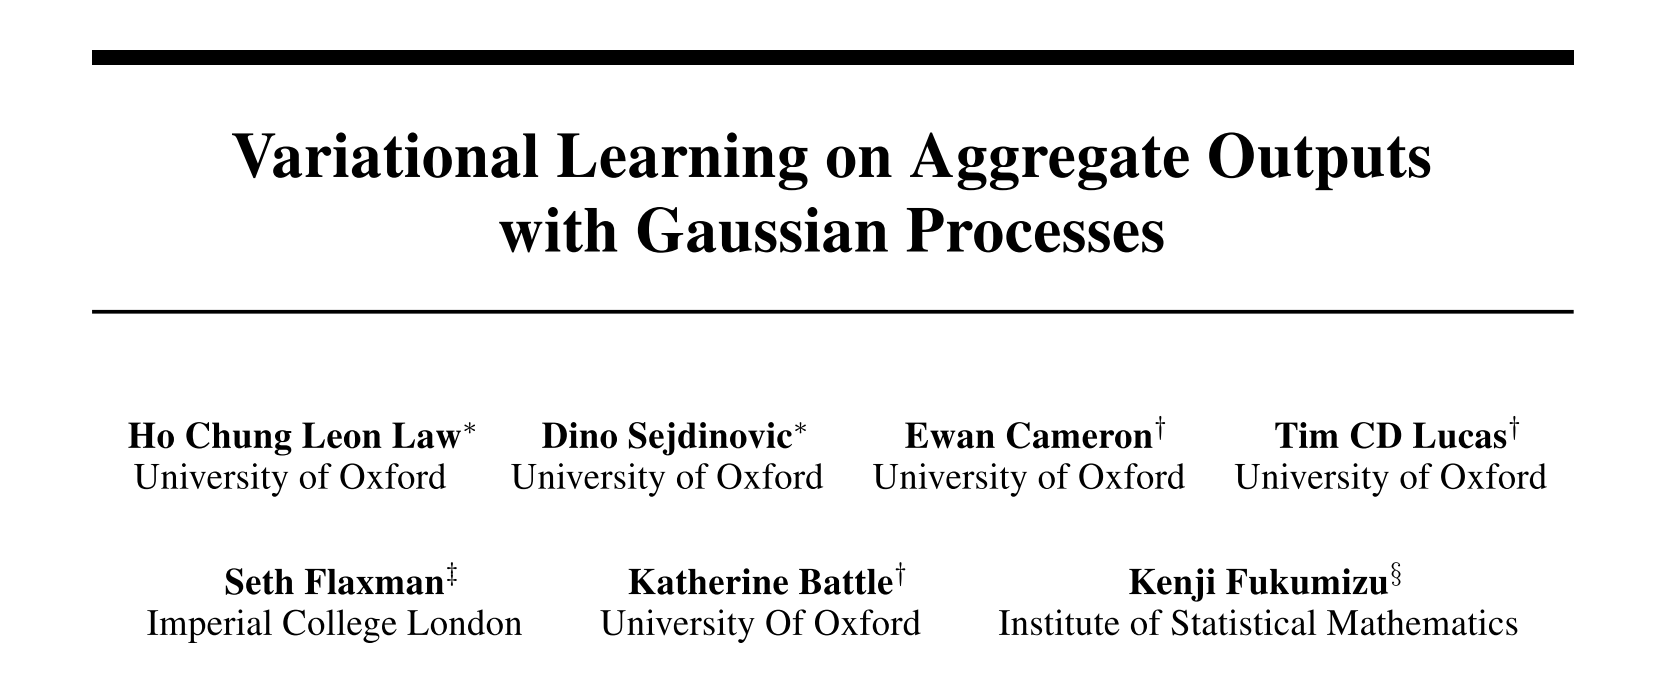
\includegraphics[width=0.4\textwidth]{photos/paper_1.png}};
	\node (fig2) at (65,-15)
	{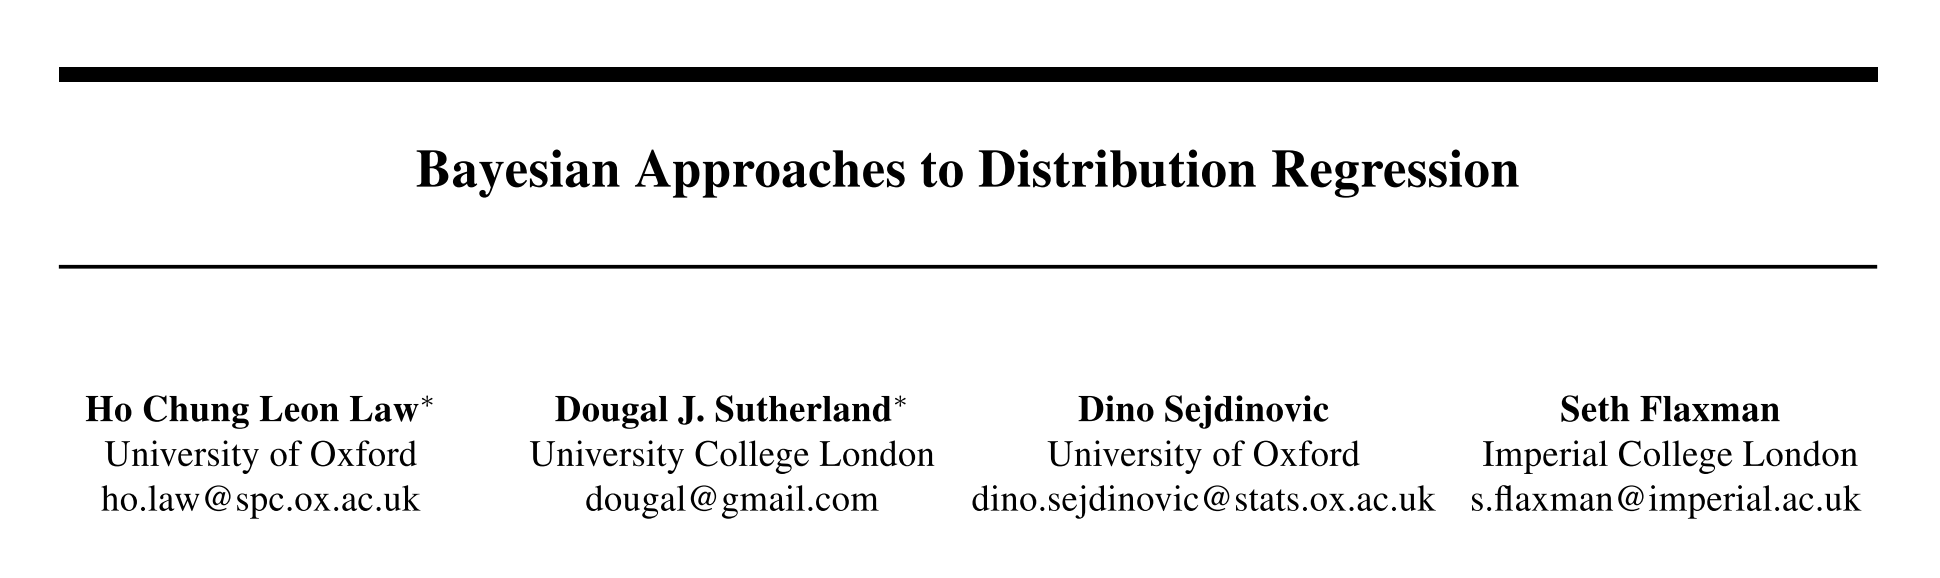
\includegraphics[width=0.45\textwidth]{photos/paper_2.png}};  
	\end{tikzpicture}
\end{figure}

\pause
\begin{itemize}
	\item \textbf{Typical supervised learning}: observe $\{\mathbf{x}_i, y_i\}_{i=1}^n$, and learn $y_i = f(\mathbf{x}_i)$
	\pause
	\item \textbf{Distribution regression}: 
	\begin{itemize}

		\item observe $\left( \{\mathbf{x}_i^1\}_{i=1}^{N_1}, y_1\right), \dots, \left( \{\mathbf{x}_i^B\}_{i=1}^{N_B}, y_B\right)$ where $\mathbf{x}_i^j \sim \mathsf{P}_j$
		\item learn $y_j = f(\mu_{\mathsf{P}_j})$, where $\mu_{\mathsf{P}_j}$ is the kernel mean embedding of $\mathsf{P}_j$ 
		\item estimate $\mu_{\mathsf{P}}$ with the empirical kernel mean embedding $\hat{\mu}_{\mathsf{P}_j} = \frac{1}{N_j}\sum_{k = 1}^{N_j} k(\cdot, x_i^j)$
	\end{itemize}
\end{itemize}
\end{frame}

\begin{frame}{A slightly different setting}

\textbf{Recall}: common problem in campaign analytics that standard techniques require survey data matched to the voterfile, which is expensive and hard to do with privacy restrictions.  Also discarding unmatched data introduces (more) bias.

\begin{center}
	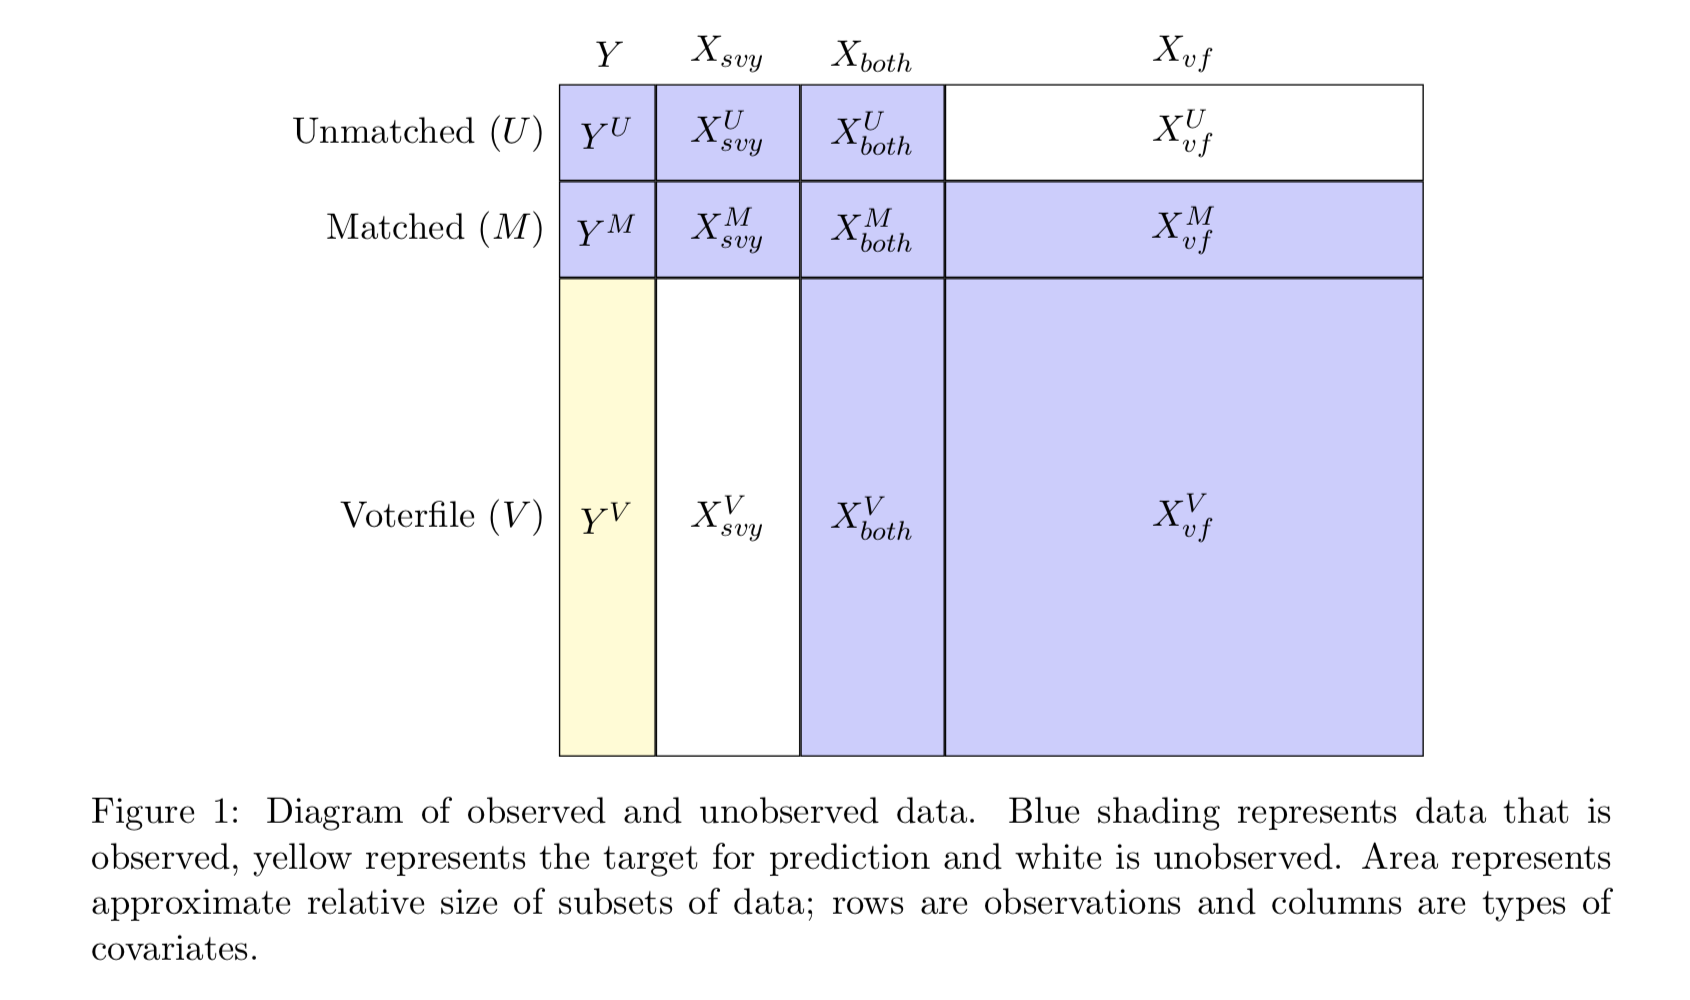
\includegraphics[width=0.8\textwidth]{photos/oursetting.png}
\end{center}

\end{frame}

\begin{frame}{Approach 1}

Key difference between this setting and standard distribution regression setting, we observe individual $y_i$, we just can't match them to covariates. 

\textbf{Idea}: Aggregate $y_i$ to move to the traditional distribution regression setting\pause
\begin{enumerate}
	\item Define $B$ bags with $X_{both}$ using \texttt{k-means++}
	\item Aggregate $y_i$ within those bags (mean or frequency counts)
	\item Embed bagged $\left(X_{both}, X_{vf}\right)$ in RKHS and calculate mean embedding
	\item Perform reglarized regression of aggregated $\bar{y}_i$ on mean embeddings
\end{enumerate}

\pause
\textbf{Variations}:
\begin{enumerate}
	\item Weighted aggregation of $y_i$ using kernel mean matching (KMM)
	\item Only aggregate unmatched $y_i$ (avoid information loss from aggregation)
\end{enumerate}


\end{frame}

\begin{frame}{Approach 1 - Simulation results}
\textbf{Data}: 5,259 responses from 4 Pew Research surveys run May-Sept 2018

\textbf{Outcome}: 3-way support for generic Dem, Rep, or Other/Not voting

\textbf{Simulation}: Fix probabilities of missingness and matching as a function of covariates.  Sample 2,000 ``respondents", then sample subset to match to the file (prop to generated probabilities). 

\begin{figure}
	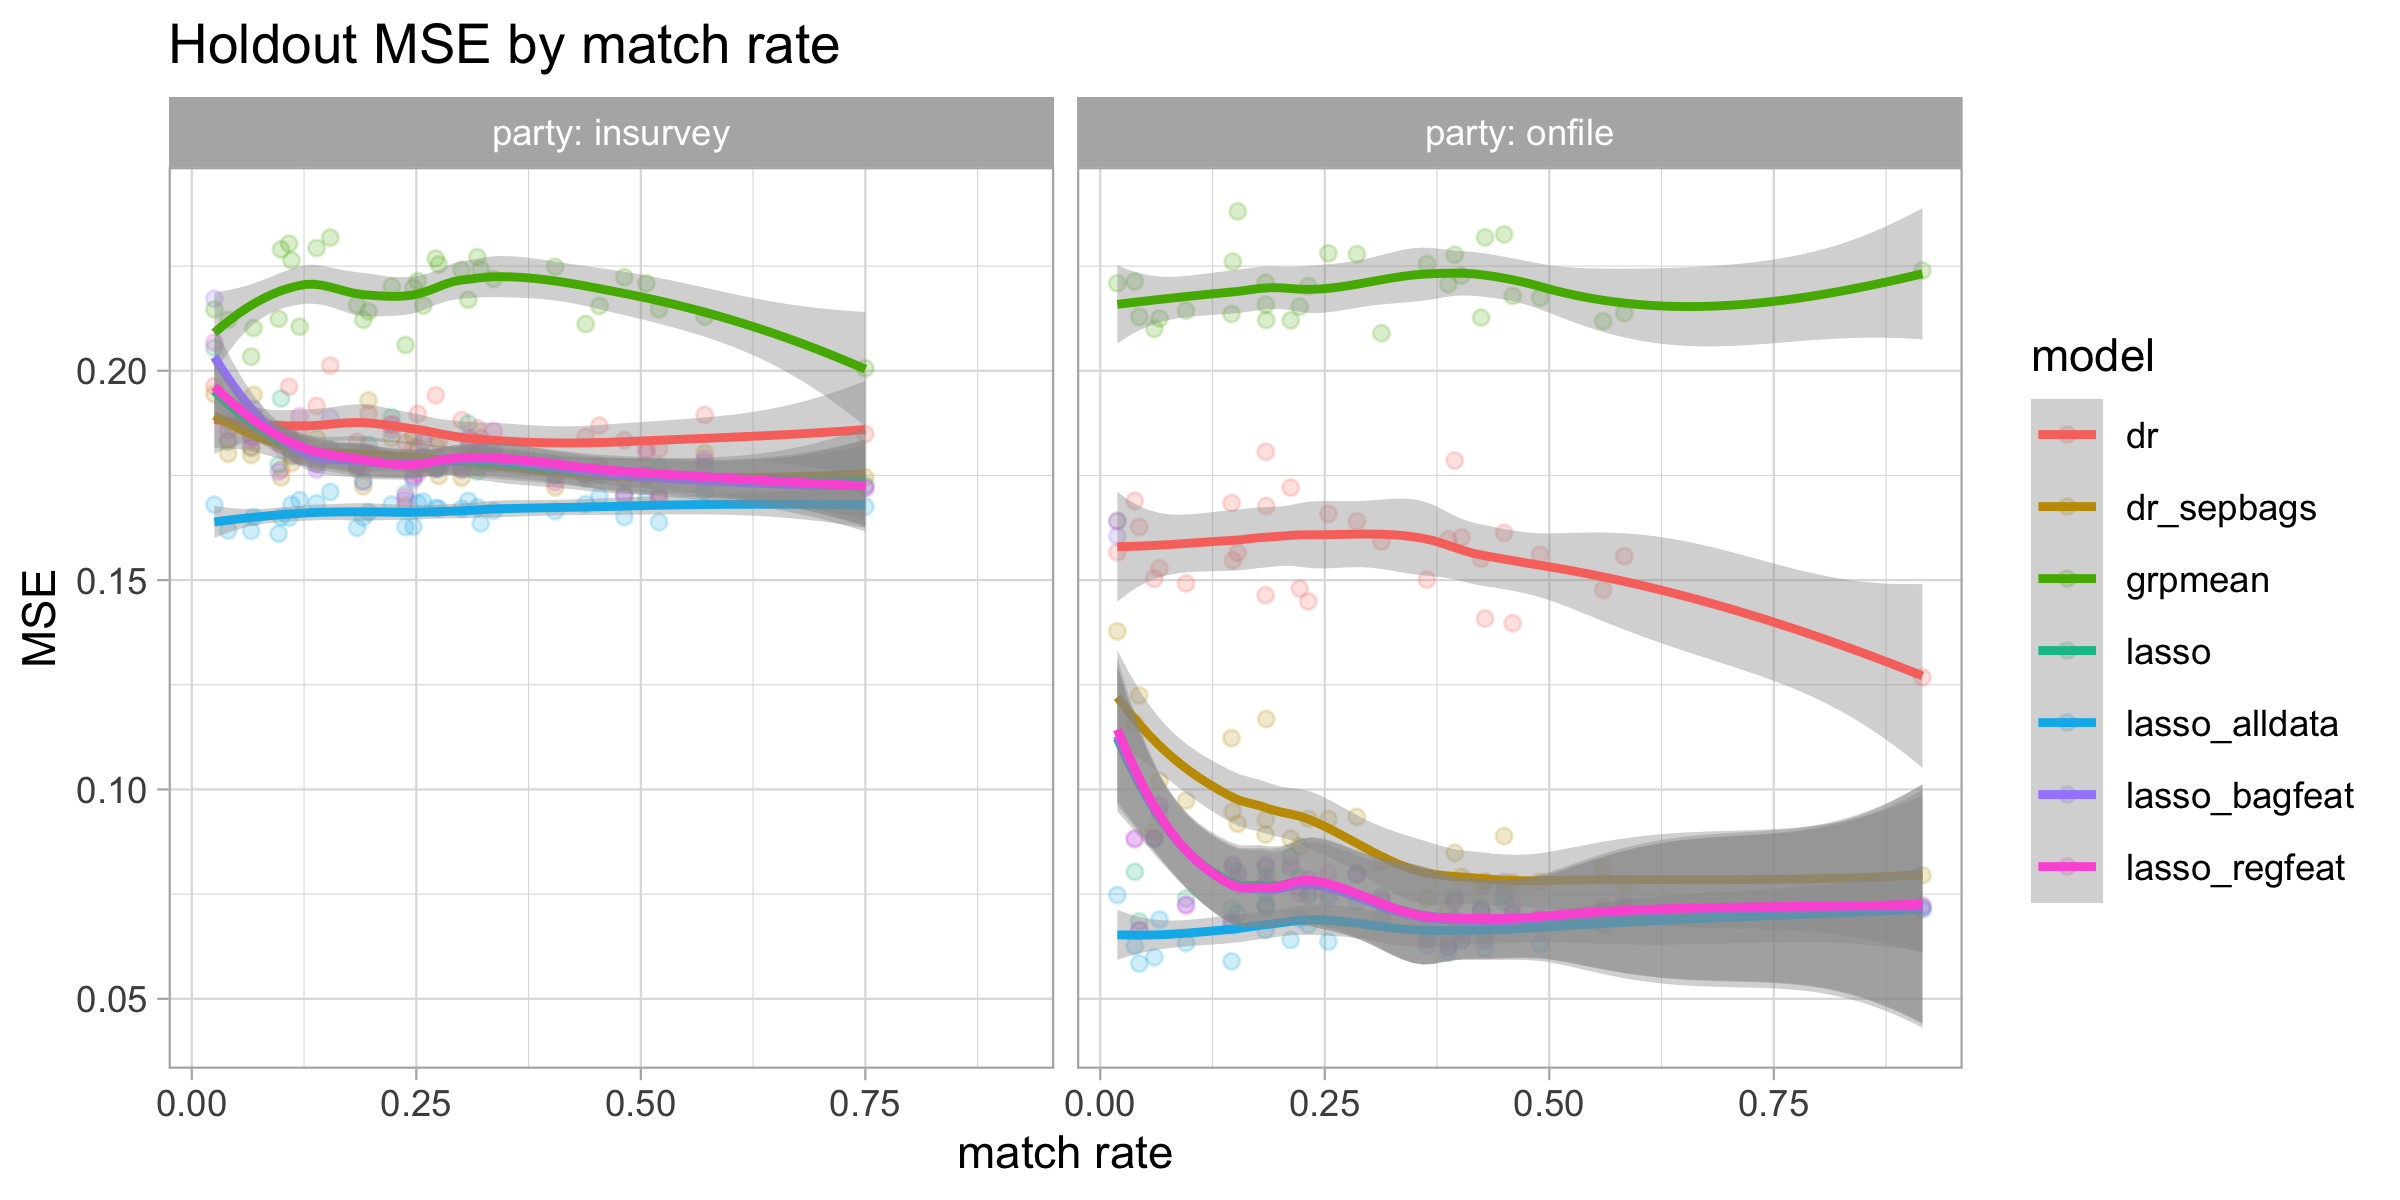
\includegraphics[width=0.8\textwidth]{~/github/bdr/pew-experiment/results/sim_randparams_v2/plots/plot_matchrate_mse.png}
\end{figure}
\end{frame}

\begin{frame}{Other approaches}
\pause
\textbf{Impute $X_{vf}^U$ with conditional VAE}:  
\begin{enumerate}
	\item Use matched data to generate realistic observations of $X_{vf}^U$ conditional on data observed in the survey $\left(Y^U, X_{svy}^U, X_{both}^U\right)$.  
	\item Then, fit normal supervised learning method on matched AND imputed data.
\end{enumerate}

\pause
\textbf{Ecological features}: Emulate hierarchical stucture of MRP with embeddings of distributional features
$$Y_i^j = \alpha f(X_i^j) + (1- \alpha)f(\mu_{\mathsf{P}_j})$$
where $\alpha$ controls weight of population v. individual-level features


\end{frame}

\section{There's (always) an election!}

\begin{frame}{T-27 Days}
\begin{figure}
	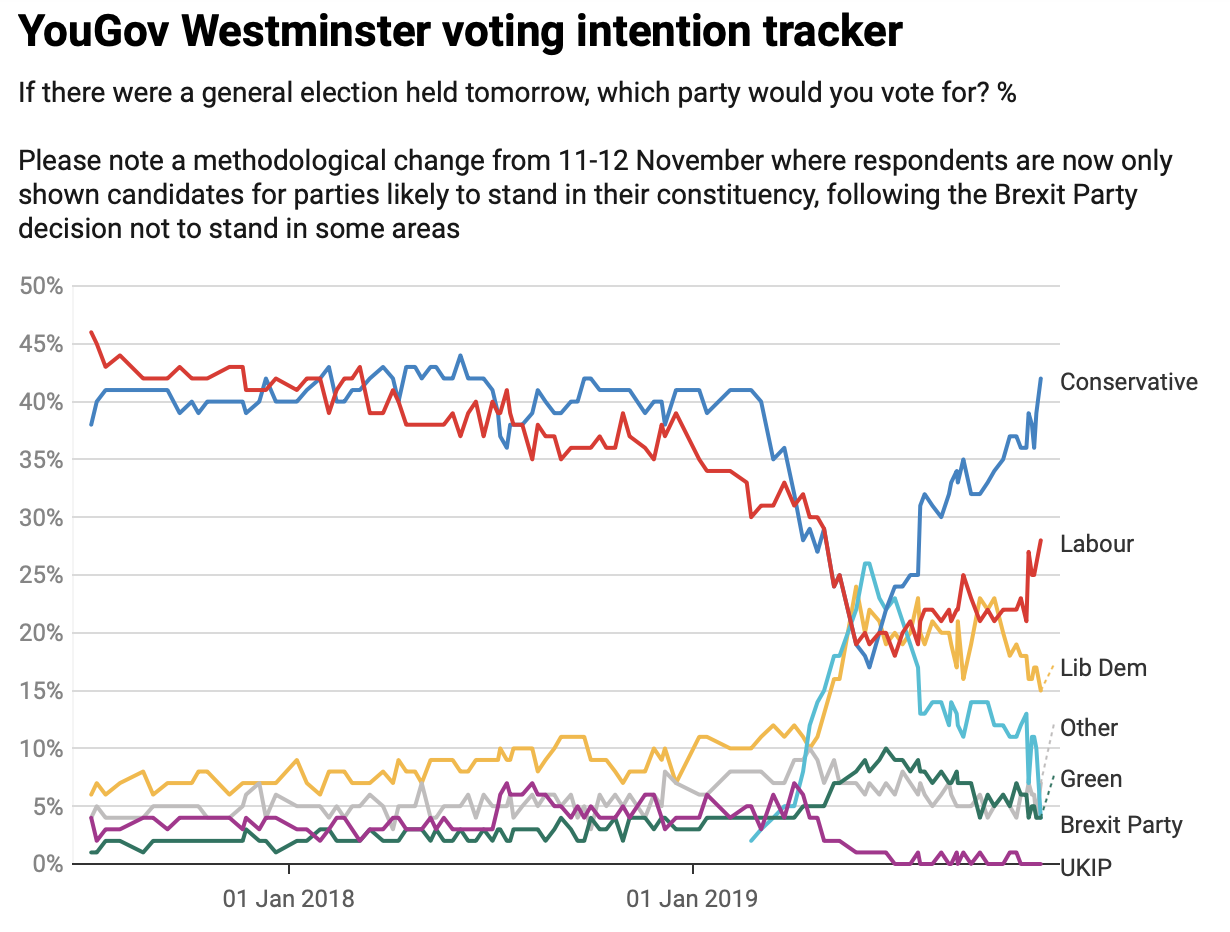
\includegraphics[width=0.5\textwidth]{photos/yougov_ge2019.png}
\end{figure}

Some interesting challenges:
\begin{itemize}
	\tightlist
	\item Tactical voting
	\item Lots of fluidity / some party re-alignment due to Brexit
	\item Even more privacy restrictions in the UK...basically \textbf{no} matched data
	\item Less advanced analytics infrastructure, very little vote history data
\end{itemize}
\end{frame}

\begin{frame}
\begin{figure}
	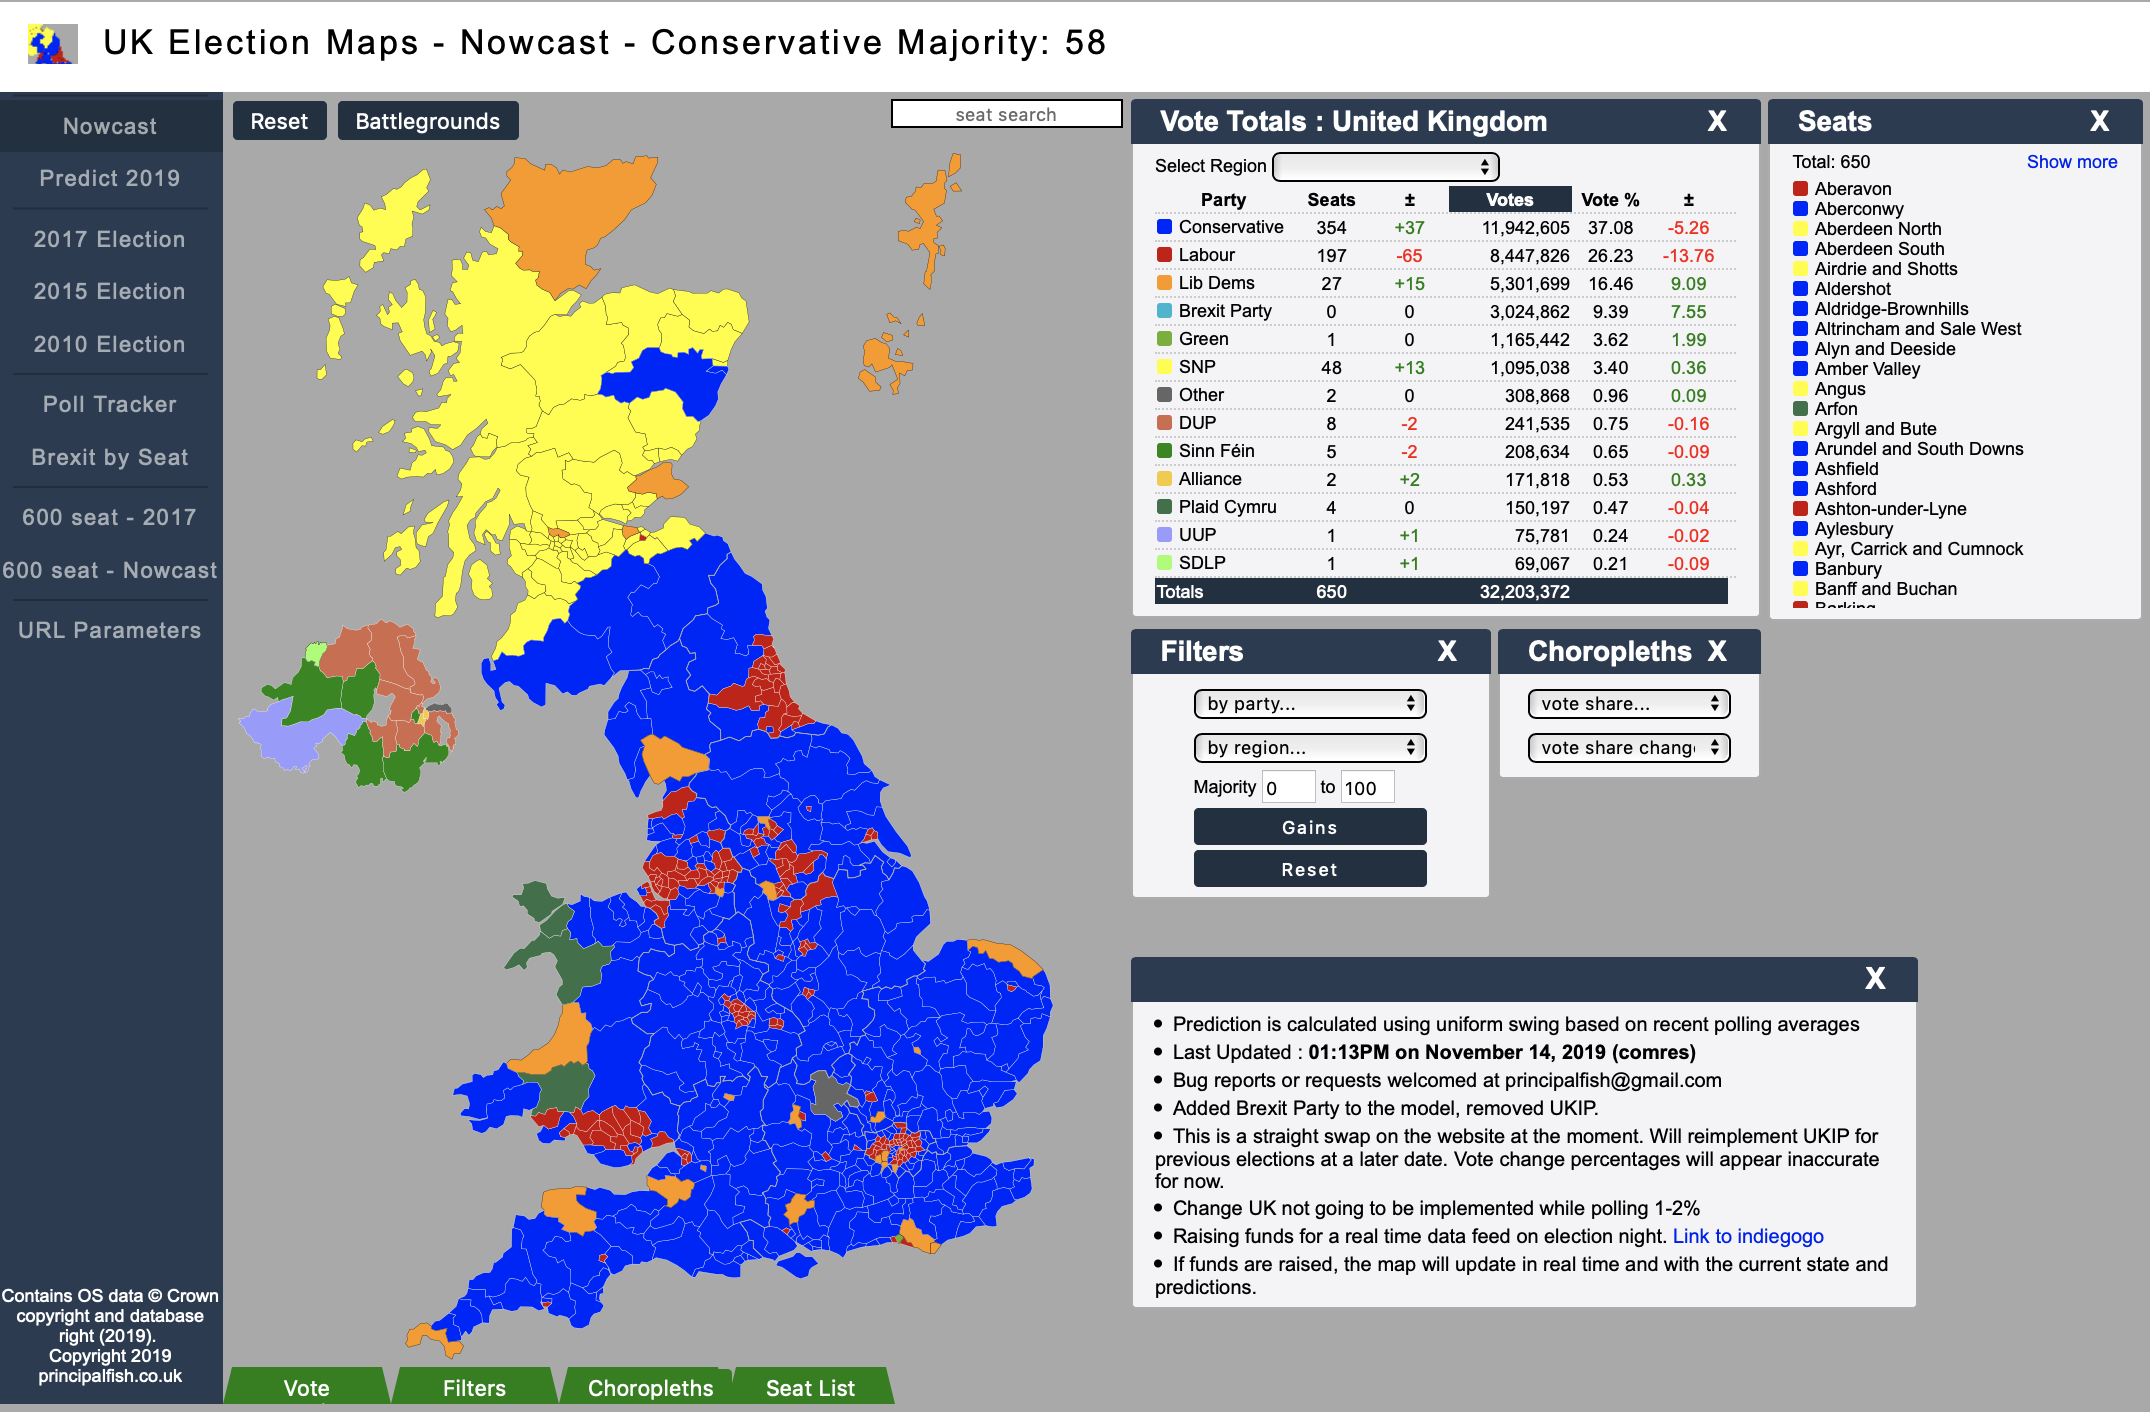
\includegraphics[width=\textwidth]{photos/principalfish_projection.png}
	\end{figure}

\small
\href{http://principalfish.co.uk/electionmaps/?map=prediction}{http://principalfish.co.uk/electionmaps/?map=prediction}
\end{frame}



\end{document}
